\documentclass[1p]{elsarticle_modified}
%\bibliographystyle{elsarticle-num}

%\usepackage[colorlinks]{hyperref}
%\usepackage{abbrmath_seonhwa} %\Abb, \Ascr, \Acal ,\Abf, \Afrak
\usepackage{amsfonts}
\usepackage{amssymb}
\usepackage{amsmath}
\usepackage{amsthm}
\usepackage{scalefnt}
\usepackage{amsbsy}
\usepackage{kotex}
\usepackage{caption}
\usepackage{subfig}
\usepackage{color}
\usepackage{graphicx}
\usepackage{xcolor} %% white, black, red, green, blue, cyan, magenta, yellow
\usepackage{float}
\usepackage{setspace}
\usepackage{hyperref}

\usepackage{tikz}
\usetikzlibrary{arrows}

\usepackage{multirow}
\usepackage{array} % fixed length table
\usepackage{hhline}

%%%%%%%%%%%%%%%%%%%%%
\makeatletter
\renewcommand*\env@matrix[1][\arraystretch]{%
	\edef\arraystretch{#1}%
	\hskip -\arraycolsep
	\let\@ifnextchar\new@ifnextchar
	\array{*\c@MaxMatrixCols c}}
\makeatother %https://tex.stackexchange.com/questions/14071/how-can-i-increase-the-line-spacing-in-a-matrix
%%%%%%%%%%%%%%%

\usepackage[normalem]{ulem}

\newcommand{\msout}[1]{\ifmmode\text{\sout{\ensuremath{#1}}}\else\sout{#1}\fi}
%SOURCE: \msout is \stkout macro in https://tex.stackexchange.com/questions/20609/strikeout-in-math-mode

\newcommand{\cancel}[1]{
	\ifmmode
	{\color{red}\msout{#1}}
	\else
	{\color{red}\sout{#1}}
	\fi
}

\newcommand{\add}[1]{
	{\color{blue}\uwave{#1}}
}

\newcommand{\replace}[2]{
	\ifmmode
	{\color{red}\msout{#1}}{\color{blue}\uwave{#2}}
	\else
	{\color{red}\sout{#1}}{\color{blue}\uwave{#2}}
	\fi
}

\newcommand{\Sol}{\mathcal{S}} %segment
\newcommand{\D}{D} %diagram
\newcommand{\A}{\mathcal{A}} %arc


%%%%%%%%%%%%%%%%%%%%%%%%%%%%%5 test

\def\sl{\operatorname{\textup{SL}}(2,\Cbb)}
\def\psl{\operatorname{\textup{PSL}}(2,\Cbb)}
\def\quan{\mkern 1mu \triangleright \mkern 1mu}

\theoremstyle{definition}
\newtheorem{thm}{Theorem}[section]
\newtheorem{prop}[thm]{Proposition}
\newtheorem{lem}[thm]{Lemma}
\newtheorem{ques}[thm]{Question}
\newtheorem{cor}[thm]{Corollary}
\newtheorem{defn}[thm]{Definition}
\newtheorem{exam}[thm]{Example}
\newtheorem{rmk}[thm]{Remark}
\newtheorem{alg}[thm]{Algorithm}

\newcommand{\I}{\sqrt{-1}}
\begin{document}

%\begin{frontmatter}
%
%\title{Boundary parabolic representations of knots up to 8 crossings}
%
%%% Group authors per affiliation:
%\author{Yunhi Cho} 
%\address{Department of Mathematics, University of Seoul, Seoul, Korea}
%\ead{yhcho@uos.ac.kr}
%
%
%\author{Seonhwa Kim} %\fnref{s_kim}}
%\address{Center for Geometry and Physics, Institute for Basic Science, Pohang, 37673, Korea}
%\ead{ryeona17@ibs.re.kr}
%
%\author{Hyuk Kim}
%\address{Department of Mathematical Sciences, Seoul National University, Seoul 08826, Korea}
%\ead{hyukkim@snu.ac.kr}
%
%\author{Seokbeom Yoon}
%\address{Department of Mathematical Sciences, Seoul National University, Seoul, 08826,  Korea}
%\ead{sbyoon15@snu.ac.kr}
%
%\begin{abstract}
%We find all boundary parabolic representation of knots up to 8 crossings.
%
%\end{abstract}
%\begin{keyword}
%    \MSC[2010] 57M25 
%\end{keyword}
%
%\end{frontmatter}

%\linenumbers
%\tableofcontents
%
\newcommand\colored[1]{\textcolor{white}{\rule[-0.35ex]{0.8em}{1.4ex}}\kern-0.8em\color{red} #1}%
%\newcommand\colored[1]{\textcolor{white}{ #1}\kern-2.17ex	\textcolor{white}{ #1}\kern-1.81ex	\textcolor{white}{ #1}\kern-2.15ex\color{red}#1	}

{\Large $\underline{12a_{0023}~(K12a_{0023})}$}

\setlength{\tabcolsep}{10pt}
\renewcommand{\arraystretch}{1.6}
\vspace{1cm}\begin{tabular}{m{100pt}>{\centering\arraybackslash}m{274pt}}
\multirow{5}{120pt}{
	\centering
	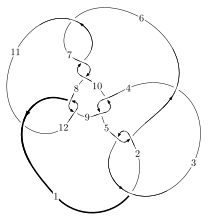
\includegraphics[width=112pt]{../../../GIT/diagram.site/Diagrams/png/824_12a_0023.png}\\
\ \ \ A knot diagram\footnotemark}&
\allowdisplaybreaks
\textbf{Linearized knot diagam} \\
\cline{2-2}
 &
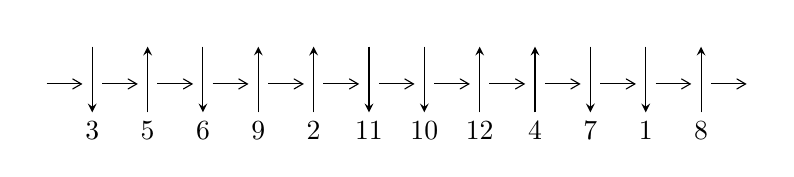
\begin{tikzpicture}[x=20pt, y=17pt]
	% nodes
	\node (C0) at (0, 0) {};
	\node (C1) at (1, 0) {};
	\node (C1U) at (1, +1) {};
	\node (C1D) at (1, -1) {3};

	\node (C2) at (2, 0) {};
	\node (C2U) at (2, +1) {};
	\node (C2D) at (2, -1) {5};

	\node (C3) at (3, 0) {};
	\node (C3U) at (3, +1) {};
	\node (C3D) at (3, -1) {6};

	\node (C4) at (4, 0) {};
	\node (C4U) at (4, +1) {};
	\node (C4D) at (4, -1) {9};

	\node (C5) at (5, 0) {};
	\node (C5U) at (5, +1) {};
	\node (C5D) at (5, -1) {2};

	\node (C6) at (6, 0) {};
	\node (C6U) at (6, +1) {};
	\node (C6D) at (6, -1) {11};

	\node (C7) at (7, 0) {};
	\node (C7U) at (7, +1) {};
	\node (C7D) at (7, -1) {10};

	\node (C8) at (8, 0) {};
	\node (C8U) at (8, +1) {};
	\node (C8D) at (8, -1) {12};

	\node (C9) at (9, 0) {};
	\node (C9U) at (9, +1) {};
	\node (C9D) at (9, -1) {4};

	\node (C10) at (10, 0) {};
	\node (C10U) at (10, +1) {};
	\node (C10D) at (10, -1) {7};

	\node (C11) at (11, 0) {};
	\node (C11U) at (11, +1) {};
	\node (C11D) at (11, -1) {1};

	\node (C12) at (12, 0) {};
	\node (C12U) at (12, +1) {};
	\node (C12D) at (12, -1) {8};
	\node (C13) at (13, 0) {};

	% arrows
	\draw[->,>={angle 60}]
	(C0) edge (C1) (C1) edge (C2) (C2) edge (C3) (C3) edge (C4) (C4) edge (C5) (C5) edge (C6) (C6) edge (C7) (C7) edge (C8) (C8) edge (C9) (C9) edge (C10) (C10) edge (C11) (C11) edge (C12) (C12) edge (C13) ;	\draw[->,>=stealth]
	(C1U) edge (C1D) (C2D) edge (C2U) (C3U) edge (C3D) (C4D) edge (C4U) (C5D) edge (C5U) (C6U) edge (C6D) (C7U) edge (C7D) (C8D) edge (C8U) (C9D) edge (C9U) (C10U) edge (C10D) (C11U) edge (C11D) (C12D) edge (C12U) ;
	\end{tikzpicture} \\
\hhline{~~} \\& 
\textbf{Solving Sequence} \\ \cline{2-2} 
 &
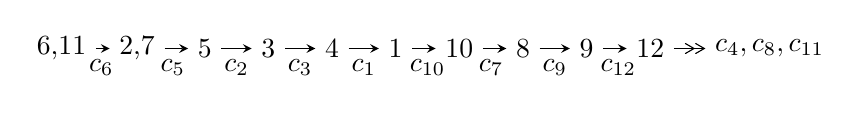
\begin{tikzpicture}[x=23pt, y=7pt]
	% node
	\node (A0) at (-1/8, 0) {6,11};
	\node (A1) at (17/16, 0) {2,7};
	\node (A2) at (17/8, 0) {5};
	\node (A3) at (25/8, 0) {3};
	\node (A4) at (33/8, 0) {4};
	\node (A5) at (41/8, 0) {1};
	\node (A6) at (49/8, 0) {10};
	\node (A7) at (57/8, 0) {8};
	\node (A8) at (65/8, 0) {9};
	\node (A9) at (73/8, 0) {12};
	\node (C1) at (1/2, -1) {$c_{6}$};
	\node (C2) at (13/8, -1) {$c_{5}$};
	\node (C3) at (21/8, -1) {$c_{2}$};
	\node (C4) at (29/8, -1) {$c_{3}$};
	\node (C5) at (37/8, -1) {$c_{1}$};
	\node (C6) at (45/8, -1) {$c_{10}$};
	\node (C7) at (53/8, -1) {$c_{7}$};
	\node (C8) at (61/8, -1) {$c_{9}$};
	\node (C9) at (69/8, -1) {$c_{12}$};
	\node (A10) at (11, 0) {$c_{4},c_{8},c_{11}$};

	% edge
	\draw[->,>=stealth]	
	(A0) edge (A1) (A1) edge (A2) (A2) edge (A3) (A3) edge (A4) (A4) edge (A5) (A5) edge (A6) (A6) edge (A7) (A7) edge (A8) (A8) edge (A9) ;
	\draw[->>,>={angle 60}]	
	(A9) edge (A10);
\end{tikzpicture} \\ 

\end{tabular} \\

\footnotetext{
The image of knot diagram is generated by the software ``\textbf{Draw programme}" developed by Andrew Bartholomew(\url{http://www.layer8.co.uk/maths/draw/index.htm\#Running-draw}), where we modified some parts for our purpose(\url{https://github.com/CATsTAILs/LinksPainter}).
}\phantom \\ \newline 
\centering \textbf{Ideals for irreducible components\footnotemark of $X_{\text{par}}$} 
 
\begin{align*}
I^u_{1}&=\langle 
1.54404\times10^{97} u^{81}-3.41633\times10^{97} u^{80}+\cdots+2.29518\times10^{98} b-3.85065\times10^{98},\\
\phantom{I^u_{1}}&\phantom{= \langle  }-1.38710\times10^{99} u^{81}+4.21392\times10^{99} u^{80}+\cdots+3.35096\times10^{100} a+5.51614\times10^{101},\\
\phantom{I^u_{1}}&\phantom{= \langle  }u^{82}-3 u^{81}+\cdots-360 u+73\rangle \\
I^u_{2}&=\langle 
- u^6-2 u^4- u^3- u^2+b- u-1,\;u^{10}+3 u^8+2 u^7+3 u^6+4 u^5+3 u^4+3 u^3+2 u^2+a+u,\\
\phantom{I^u_{2}}&\phantom{= \langle  }u^{12}+4 u^{10}+2 u^9+6 u^8+6 u^7+7 u^6+6 u^5+7 u^4+3 u^3+3 u^2+u+1\rangle \\
I^u_{3}&=\langle 
u^2 a- a u+u^2+b- u,\;2 u^3 a-4 u^2 a-5 u^3+4 a^2+6 a u+6 u^2-2 a-13 u+15,\;u^4- u^3+3 u^2-2 u+1\rangle \\
I^u_{4}&=\langle 
89 a^4 u+27 a^4-332 a^3 u+255 a^3+238 a^2 u-336 a^2-693 a u+173 b+93 a+205 u-208,\\
\phantom{I^u_{4}}&\phantom{= \langle  }a^5-5 a^4 u-4 a^4+13 a^3 u-12 a^2 u-2 a^2+18 a u+3 a-6 u+5,\;u^2+1\rangle \\
I^u_{5}&=\langle 
u^{12}+4 u^{10}+2 u^9+6 u^8+6 u^7+6 u^6+6 u^5+5 u^4+2 u^3+2 u^2+b,\\
\phantom{I^u_{5}}&\phantom{= \langle  }u^{12}+5 u^{10}+2 u^9+9 u^8+8 u^7+10 u^6+10 u^5+10 u^4+6 u^3+5 u^2+a+2 u+1,\;u^{18}+6 u^{16}+\cdots+2 u^3+1\rangle \\
\\
\end{align*}
\raggedright * 5 irreducible components of $\dim_{\mathbb{C}}=0$, with total 130 representations.\\
\footnotetext{All coefficients of polynomials are rational numbers. But the coefficients are sometimes approximated in decimal forms when there is not enough margin.}
\newpage
\renewcommand{\arraystretch}{1}
\centering \section*{I. $I^u_{1}= \langle 1.54\times10^{97} u^{81}-3.42\times10^{97} u^{80}+\cdots+2.30\times10^{98} b-3.85\times10^{98},\;-1.39\times10^{99} u^{81}+4.21\times10^{99} u^{80}+\cdots+3.35\times10^{100} a+5.52\times10^{101},\;u^{82}-3 u^{81}+\cdots-360 u+73 \rangle$}
\flushleft \textbf{(i) Arc colorings}\\
\begin{tabular}{m{7pt} m{180pt} m{7pt} m{180pt} }
\flushright $a_{6}=$&$\begin{pmatrix}1\\0\end{pmatrix}$ \\
\flushright $a_{11}=$&$\begin{pmatrix}0\\u\end{pmatrix}$ \\
\flushright $a_{2}=$&$\begin{pmatrix}0.0413941 u^{81}-0.125753 u^{80}+\cdots+42.8841 u-16.4614\\-0.0672732 u^{81}+0.148848 u^{80}+\cdots-8.13184 u+1.67771\end{pmatrix}$ \\
\flushright $a_{7}=$&$\begin{pmatrix}1\\u^2\end{pmatrix}$ \\
\flushright $a_{5}=$&$\begin{pmatrix}-0.0821417 u^{81}+0.264163 u^{80}+\cdots-69.1648 u+27.9833\\0.128564 u^{81}-0.295774 u^{80}+\cdots+10.3237 u-0.432825\end{pmatrix}$ \\
\flushright $a_{3}=$&$\begin{pmatrix}0.129775 u^{81}-0.321359 u^{80}+\cdots+96.0521 u-36.0885\\-0.134314 u^{81}+0.328329 u^{80}+\cdots-16.2930 u+0.328601\end{pmatrix}$ \\
\flushright $a_{4}=$&$\begin{pmatrix}0.264088 u^{81}-0.649687 u^{80}+\cdots+112.345 u-36.4171\\-0.134314 u^{81}+0.328329 u^{80}+\cdots-16.2930 u+0.328601\end{pmatrix}$ \\
\flushright $a_{1}=$&$\begin{pmatrix}0.0708172 u^{81}-0.216816 u^{80}+\cdots+43.2679 u-15.8971\\-0.0495787 u^{81}+0.0950525 u^{80}+\cdots-4.54197 u+2.12782\end{pmatrix}$ \\
\flushright $a_{10}=$&$\begin{pmatrix}u\\u^3+u\end{pmatrix}$ \\
\flushright $a_{8}=$&$\begin{pmatrix}u^2+1\\u^4+2 u^2\end{pmatrix}$ \\
\flushright $a_{9}=$&$\begin{pmatrix}0.0784673 u^{81}-0.196720 u^{80}+\cdots+47.2231 u-14.7403\\0.0892485 u^{81}-0.257911 u^{80}+\cdots+33.5150 u-11.6127\end{pmatrix}$ \\
\flushright $a_{12}=$&$\begin{pmatrix}0.153951 u^{81}-0.394472 u^{80}+\cdots+69.7949 u-26.5441\\-0.00512662 u^{81}-0.00648671 u^{80}+\cdots+9.47710 u-2.79106\end{pmatrix}$\\&\end{tabular}
\flushleft \textbf{(ii) Obstruction class $= -1$}\\~\\
\flushleft \textbf{(iii) Cusp Shapes $= 0.0994831 u^{81}-0.402830 u^{80}+\cdots-10.5235 u+2.17824$}\\~\\
\newpage\renewcommand{\arraystretch}{1}
\flushleft \textbf{(iv) u-Polynomials at the component}\newline \\
\begin{tabular}{m{50pt}|m{274pt}}
Crossings & \hspace{64pt}u-Polynomials at each crossing \\
\hline $$\begin{aligned}c_{1}\end{aligned}$$&$\begin{aligned}
&u^{82}+40 u^{81}+\cdots-49 u+16
\end{aligned}$\\
\hline $$\begin{aligned}c_{2},c_{5}\end{aligned}$$&$\begin{aligned}
&u^{82}+4 u^{81}+\cdots+35 u+4
\end{aligned}$\\
\hline $$\begin{aligned}c_{3}\end{aligned}$$&$\begin{aligned}
&u^{82}-4 u^{81}+\cdots+198067 u+62564
\end{aligned}$\\
\hline $$\begin{aligned}c_{4},c_{9}\end{aligned}$$&$\begin{aligned}
&u^{82}-2 u^{81}+\cdots-1536 u+2048
\end{aligned}$\\
\hline $$\begin{aligned}c_{6},c_{7},c_{10}\end{aligned}$$&$\begin{aligned}
&u^{82}-3 u^{81}+\cdots-360 u+73
\end{aligned}$\\
\hline $$\begin{aligned}c_{8},c_{12}\end{aligned}$$&$\begin{aligned}
&u^{82}-3 u^{81}+\cdots-494 u+73
\end{aligned}$\\
\hline $$\begin{aligned}c_{11}\end{aligned}$$&$\begin{aligned}
&u^{82}+33 u^{81}+\cdots+157464 u+5329
\end{aligned}$\\
\hline
\end{tabular}\\~\\
\newpage\renewcommand{\arraystretch}{1}
\flushleft \textbf{(v) Riley Polynomials at the component}\newline \\
\begin{tabular}{m{50pt}|m{274pt}}
Crossings & \hspace{64pt}Riley Polynomials at each crossing \\
\hline $$\begin{aligned}c_{1}\end{aligned}$$&$\begin{aligned}
&y^{82}+8 y^{81}+\cdots+20543 y+256
\end{aligned}$\\
\hline $$\begin{aligned}c_{2},c_{5}\end{aligned}$$&$\begin{aligned}
&y^{82}+40 y^{81}+\cdots-49 y+16
\end{aligned}$\\
\hline $$\begin{aligned}c_{3}\end{aligned}$$&$\begin{aligned}
&y^{82}-24 y^{81}+\cdots-66737549857 y+3914254096
\end{aligned}$\\
\hline $$\begin{aligned}c_{4},c_{9}\end{aligned}$$&$\begin{aligned}
&y^{82}+40 y^{81}+\cdots+81002496 y+4194304
\end{aligned}$\\
\hline $$\begin{aligned}c_{6},c_{7},c_{10}\end{aligned}$$&$\begin{aligned}
&y^{82}+85 y^{81}+\cdots-1704 y+5329
\end{aligned}$\\
\hline $$\begin{aligned}c_{8},c_{12}\end{aligned}$$&$\begin{aligned}
&y^{82}+33 y^{81}+\cdots+157464 y+5329
\end{aligned}$\\
\hline $$\begin{aligned}c_{11}\end{aligned}$$&$\begin{aligned}
&y^{82}+45 y^{81}+\cdots-920479712 y+28398241
\end{aligned}$\\
\hline
\end{tabular}\\~\\
\newpage\flushleft \textbf{(vi) Complex Volumes and Cusp Shapes}
$$\begin{array}{c|c|c}  
\text{Solutions to }I^u_{1}& \I (\text{vol} + \sqrt{-1}CS) & \text{Cusp shape}\\
 \hline 
\begin{aligned}
u &= \phantom{-}0.931867 + 0.288264 I \\
a &= \phantom{-}0.74456 + 2.19168 I \\
b &= -0.578133 + 1.146860 I\end{aligned}
 & -4.73439 - 13.08270 I & \phantom{-0.000000 } 0 \\ \hline\begin{aligned}
u &= \phantom{-}0.931867 - 0.288264 I \\
a &= \phantom{-}0.74456 - 2.19168 I \\
b &= -0.578133 - 1.146860 I\end{aligned}
 & -4.73439 + 13.08270 I & \phantom{-0.000000 } 0 \\ \hline\begin{aligned}
u &= -0.716067 + 0.747461 I \\
a &= -0.032611 + 1.086440 I \\
b &= -0.496263 + 1.079110 I\end{aligned}
 & -1.68085 - 2.38669 I & \phantom{-0.000000 } 0 \\ \hline\begin{aligned}
u &= -0.716067 - 0.747461 I \\
a &= -0.032611 - 1.086440 I \\
b &= -0.496263 - 1.079110 I\end{aligned}
 & -1.68085 + 2.38669 I & \phantom{-0.000000 } 0 \\ \hline\begin{aligned}
u &= \phantom{-}0.881772 + 0.288043 I \\
a &= -0.567238 + 0.105365 I \\
b &= -0.812359 - 0.318846 I\end{aligned}
 & -2.27548 - 7.90430 I & \phantom{-0.000000 } 0 \\ \hline\begin{aligned}
u &= \phantom{-}0.881772 - 0.288043 I \\
a &= -0.567238 - 0.105365 I \\
b &= -0.812359 + 0.318846 I\end{aligned}
 & -2.27548 + 7.90430 I & \phantom{-0.000000 } 0 \\ \hline\begin{aligned}
u &= -0.552972 + 0.923521 I \\
a &= \phantom{-}1.04759 - 1.44828 I \\
b &= -0.404154 - 1.082810 I\end{aligned}
 & -2.30869 + 4.66431 I & \phantom{-0.000000 } 0 \\ \hline\begin{aligned}
u &= -0.552972 - 0.923521 I \\
a &= \phantom{-}1.04759 + 1.44828 I \\
b &= -0.404154 + 1.082810 I\end{aligned}
 & -2.30869 - 4.66431 I & \phantom{-0.000000 } 0 \\ \hline\begin{aligned}
u &= \phantom{-}0.865905 + 0.193943 I \\
a &= -0.21817 - 2.33698 I \\
b &= -0.225527 - 1.181770 I\end{aligned}
 & -7.10693 - 4.86870 I & \phantom{-0.000000 } 0 \\ \hline\begin{aligned}
u &= \phantom{-}0.865905 - 0.193943 I \\
a &= -0.21817 + 2.33698 I \\
b &= -0.225527 + 1.181770 I\end{aligned}
 & -7.10693 + 4.86870 I & \phantom{-0.000000 } 0\\
 \hline 
 \end{array}$$\newpage$$\begin{array}{c|c|c}  
\text{Solutions to }I^u_{1}& \I (\text{vol} + \sqrt{-1}CS) & \text{Cusp shape}\\
 \hline 
\begin{aligned}
u &= -0.629083 + 0.592688 I \\
a &= \phantom{-}0.557418 - 0.631931 I \\
b &= -0.462219 - 0.392158 I\end{aligned}
 & \phantom{-}0.35733 + 1.72933 I & \phantom{-0.000000 } 0 \\ \hline\begin{aligned}
u &= -0.629083 - 0.592688 I \\
a &= \phantom{-}0.557418 + 0.631931 I \\
b &= -0.462219 + 0.392158 I\end{aligned}
 & \phantom{-}0.35733 - 1.72933 I & \phantom{-0.000000 } 0 \\ \hline\begin{aligned}
u &= -0.757316 + 0.260733 I \\
a &= -0.54770 + 3.02690 I \\
b &= \phantom{-}0.514202 + 1.095290 I\end{aligned}
 & -2.21702 + 6.90031 I & -3.45370 - 7.38488 I \\ \hline\begin{aligned}
u &= -0.757316 - 0.260733 I \\
a &= -0.54770 - 3.02690 I \\
b &= \phantom{-}0.514202 - 1.095290 I\end{aligned}
 & -2.21702 - 6.90031 I & -3.45370 + 7.38488 I \\ \hline\begin{aligned}
u &= \phantom{-}0.708061 + 0.318172 I \\
a &= \phantom{-}0.036016 - 0.721055 I \\
b &= \phantom{-}0.702828 - 0.691781 I\end{aligned}
 & -0.26229 - 5.35525 I & -1.75979 + 8.80201 I \\ \hline\begin{aligned}
u &= \phantom{-}0.708061 - 0.318172 I \\
a &= \phantom{-}0.036016 + 0.721055 I \\
b &= \phantom{-}0.702828 + 0.691781 I\end{aligned}
 & -0.26229 + 5.35525 I & -1.75979 - 8.80201 I \\ \hline\begin{aligned}
u &= \phantom{-}0.102266 + 1.220550 I \\
a &= \phantom{-}0.346306 - 1.356210 I \\
b &= -0.485285 - 1.241660 I\end{aligned}
 & -4.87377 + 3.17759 I & \phantom{-0.000000 } 0 \\ \hline\begin{aligned}
u &= \phantom{-}0.102266 - 1.220550 I \\
a &= \phantom{-}0.346306 + 1.356210 I \\
b &= -0.485285 + 1.241660 I\end{aligned}
 & -4.87377 - 3.17759 I & \phantom{-0.000000 } 0 \\ \hline\begin{aligned}
u &= -0.331871 + 0.700232 I \\
a &= \phantom{-}0.496451 - 0.036342 I \\
b &= -0.301233 + 0.157524 I\end{aligned}
 & \phantom{-}0.204488 + 1.398330 I & \phantom{-}2.03862 - 5.44556 I \\ \hline\begin{aligned}
u &= -0.331871 - 0.700232 I \\
a &= \phantom{-}0.496451 + 0.036342 I \\
b &= -0.301233 - 0.157524 I\end{aligned}
 & \phantom{-}0.204488 - 1.398330 I & \phantom{-}2.03862 + 5.44556 I\\
 \hline 
 \end{array}$$\newpage$$\begin{array}{c|c|c}  
\text{Solutions to }I^u_{1}& \I (\text{vol} + \sqrt{-1}CS) & \text{Cusp shape}\\
 \hline 
\begin{aligned}
u &= -0.674373 + 0.346981 I \\
a &= \phantom{-}1.073310 + 0.123315 I \\
b &= \phantom{-}0.578755 - 0.306719 I\end{aligned}
 & \phantom{-}0.00632 + 2.50124 I & \phantom{-}0.80512 - 3.77203 I \\ \hline\begin{aligned}
u &= -0.674373 - 0.346981 I \\
a &= \phantom{-}1.073310 - 0.123315 I \\
b &= \phantom{-}0.578755 + 0.306719 I\end{aligned}
 & \phantom{-}0.00632 - 2.50124 I & \phantom{-}0.80512 + 3.77203 I \\ \hline\begin{aligned}
u &= \phantom{-}0.186356 + 1.239000 I \\
a &= \phantom{-}0.56436 + 1.53697 I \\
b &= -0.407486 + 1.256420 I\end{aligned}
 & -5.40817 - 6.29101 I & \phantom{-0.000000 } 0 \\ \hline\begin{aligned}
u &= \phantom{-}0.186356 - 1.239000 I \\
a &= \phantom{-}0.56436 - 1.53697 I \\
b &= -0.407486 - 1.256420 I\end{aligned}
 & -5.40817 + 6.29101 I & \phantom{-0.000000 } 0 \\ \hline\begin{aligned}
u &= \phantom{-}0.131448 + 1.261180 I \\
a &= \phantom{-}0.0126024 + 0.1044920 I \\
b &= -0.894097 + 0.065764 I\end{aligned}
 & -1.27320 - 1.76086 I & \phantom{-0.000000 } 0 \\ \hline\begin{aligned}
u &= \phantom{-}0.131448 - 1.261180 I \\
a &= \phantom{-}0.0126024 - 0.1044920 I \\
b &= -0.894097 - 0.065764 I\end{aligned}
 & -1.27320 + 1.76086 I & \phantom{-0.000000 } 0 \\ \hline\begin{aligned}
u &= \phantom{-}0.000944 + 0.700428 I \\
a &= \phantom{-}0.836733 - 0.250241 I \\
b &= \phantom{-}0.453431 + 0.652167 I\end{aligned}
 & \phantom{-}0.85090 + 1.37273 I & \phantom{-}5.63231 - 4.46237 I \\ \hline\begin{aligned}
u &= \phantom{-}0.000944 - 0.700428 I \\
a &= \phantom{-}0.836733 + 0.250241 I \\
b &= \phantom{-}0.453431 - 0.652167 I\end{aligned}
 & \phantom{-}0.85090 - 1.37273 I & \phantom{-}5.63231 + 4.46237 I \\ \hline\begin{aligned}
u &= \phantom{-}0.600384 + 0.298134 I \\
a &= -0.26365 + 1.53064 I \\
b &= \phantom{-}0.645915 + 0.903317 I\end{aligned}
 & -0.883850 - 0.200745 I & -5.12754 + 3.53229 I \\ \hline\begin{aligned}
u &= \phantom{-}0.600384 - 0.298134 I \\
a &= -0.26365 - 1.53064 I \\
b &= \phantom{-}0.645915 - 0.903317 I\end{aligned}
 & -0.883850 + 0.200745 I & -5.12754 - 3.53229 I\\
 \hline 
 \end{array}$$\newpage$$\begin{array}{c|c|c}  
\text{Solutions to }I^u_{1}& \I (\text{vol} + \sqrt{-1}CS) & \text{Cusp shape}\\
 \hline 
\begin{aligned}
u &= \phantom{-}0.044049 + 1.339840 I \\
a &= \phantom{-}0.38952 + 1.43290 I \\
b &= \phantom{-}0.201452 + 1.108560 I\end{aligned}
 & \phantom{-}2.76790 + 2.04513 I & \phantom{-0.000000 } 0 \\ \hline\begin{aligned}
u &= \phantom{-}0.044049 - 1.339840 I \\
a &= \phantom{-}0.38952 - 1.43290 I \\
b &= \phantom{-}0.201452 - 1.108560 I\end{aligned}
 & \phantom{-}2.76790 - 2.04513 I & \phantom{-0.000000 } 0 \\ \hline\begin{aligned}
u &= \phantom{-}0.638837 + 0.095613 I \\
a &= -1.03149 - 2.03244 I \\
b &= -0.360549 - 1.188300 I\end{aligned}
 & -8.84527 + 3.38561 I & -9.80482 - 3.21851 I \\ \hline\begin{aligned}
u &= \phantom{-}0.638837 - 0.095613 I \\
a &= -1.03149 + 2.03244 I \\
b &= -0.360549 + 1.188300 I\end{aligned}
 & -8.84527 - 3.38561 I & -9.80482 + 3.21851 I \\ \hline\begin{aligned}
u &= -0.217222 + 1.359330 I \\
a &= \phantom{-}0.41987 - 1.65460 I \\
b &= \phantom{-}0.309949 - 1.160650 I\end{aligned}
 & \phantom{-}1.51647 + 2.63898 I & \phantom{-0.000000 } 0 \\ \hline\begin{aligned}
u &= -0.217222 - 1.359330 I \\
a &= \phantom{-}0.41987 + 1.65460 I \\
b &= \phantom{-}0.309949 + 1.160650 I\end{aligned}
 & \phantom{-}1.51647 - 2.63898 I & \phantom{-0.000000 } 0 \\ \hline\begin{aligned}
u &= -0.580389 + 0.144752 I \\
a &= -0.08898 - 3.84967 I \\
b &= \phantom{-}0.368006 - 1.071140 I\end{aligned}
 & -3.26708 - 0.25890 I & -6.56949 - 0.34009 I \\ \hline\begin{aligned}
u &= -0.580389 - 0.144752 I \\
a &= -0.08898 + 3.84967 I \\
b &= \phantom{-}0.368006 + 1.071140 I\end{aligned}
 & -3.26708 + 0.25890 I & -6.56949 + 0.34009 I \\ \hline\begin{aligned}
u &= -0.293167 + 1.373670 I \\
a &= -0.364644 + 0.989732 I \\
b &= -0.155107 + 1.157470 I\end{aligned}
 & \phantom{-}0.62942 + 3.86909 I & \phantom{-0.000000 } 0 \\ \hline\begin{aligned}
u &= -0.293167 - 1.373670 I \\
a &= -0.364644 - 0.989732 I \\
b &= -0.155107 - 1.157470 I\end{aligned}
 & \phantom{-}0.62942 - 3.86909 I & \phantom{-0.000000 } 0\\
 \hline 
 \end{array}$$\newpage$$\begin{array}{c|c|c}  
\text{Solutions to }I^u_{1}& \I (\text{vol} + \sqrt{-1}CS) & \text{Cusp shape}\\
 \hline 
\begin{aligned}
u &= -0.10157 + 1.41564 I \\
a &= -1.007610 - 0.291358 I \\
b &= \phantom{-}0.672906 - 0.991984 I\end{aligned}
 & \phantom{-}6.01806 - 2.03585 I & \phantom{-0.000000 } 0 \\ \hline\begin{aligned}
u &= -0.10157 - 1.41564 I \\
a &= -1.007610 + 0.291358 I \\
b &= \phantom{-}0.672906 + 0.991984 I\end{aligned}
 & \phantom{-}6.01806 + 2.03585 I & \phantom{-0.000000 } 0 \\ \hline\begin{aligned}
u &= \phantom{-}0.19353 + 1.40902 I \\
a &= -1.56362 - 1.41156 I \\
b &= \phantom{-}0.571655 - 1.099770 I\end{aligned}
 & \phantom{-}5.20020 - 5.30195 I & \phantom{-0.000000 } 0 \\ \hline\begin{aligned}
u &= \phantom{-}0.19353 - 1.40902 I \\
a &= -1.56362 + 1.41156 I \\
b &= \phantom{-}0.571655 + 1.099770 I\end{aligned}
 & \phantom{-}5.20020 + 5.30195 I & \phantom{-0.000000 } 0 \\ \hline\begin{aligned}
u &= \phantom{-}0.23431 + 1.41260 I \\
a &= -0.563863 + 0.112880 I \\
b &= \phantom{-}0.720598 + 0.946524 I\end{aligned}
 & \phantom{-}4.58279 - 3.27171 I & \phantom{-0.000000 } 0 \\ \hline\begin{aligned}
u &= \phantom{-}0.23431 - 1.41260 I \\
a &= -0.563863 - 0.112880 I \\
b &= \phantom{-}0.720598 - 0.946524 I\end{aligned}
 & \phantom{-}4.58279 + 3.27171 I & \phantom{-0.000000 } 0 \\ \hline\begin{aligned}
u &= \phantom{-}0.141385 + 0.546620 I \\
a &= -1.17091 - 2.94774 I \\
b &= \phantom{-}0.537230 - 0.935250 I\end{aligned}
 & \phantom{-}0.01009 - 2.82413 I & \phantom{-}1.52552 - 1.31964 I \\ \hline\begin{aligned}
u &= \phantom{-}0.141385 - 0.546620 I \\
a &= -1.17091 + 2.94774 I \\
b &= \phantom{-}0.537230 + 0.935250 I\end{aligned}
 & \phantom{-}0.01009 + 2.82413 I & \phantom{-}1.52552 + 1.31964 I \\ \hline\begin{aligned}
u &= \phantom{-}0.35574 + 1.39551 I \\
a &= -0.589303 - 1.191880 I \\
b &= -0.181803 - 1.231480 I\end{aligned}
 & -2.06157 - 9.25202 I & \phantom{-0.000000 } 0 \\ \hline\begin{aligned}
u &= \phantom{-}0.35574 - 1.39551 I \\
a &= -0.589303 + 1.191880 I \\
b &= -0.181803 + 1.231480 I\end{aligned}
 & -2.06157 + 9.25202 I & \phantom{-0.000000 } 0\\
 \hline 
 \end{array}$$\newpage$$\begin{array}{c|c|c}  
\text{Solutions to }I^u_{1}& \I (\text{vol} + \sqrt{-1}CS) & \text{Cusp shape}\\
 \hline 
\begin{aligned}
u &= -0.15745 + 1.43439 I \\
a &= -0.807625 - 0.077038 I \\
b &= \phantom{-}0.768058 + 0.620750 I\end{aligned}
 & \phantom{-}7.11638 + 3.39177 I & \phantom{-0.000000 } 0 \\ \hline\begin{aligned}
u &= -0.15745 - 1.43439 I \\
a &= -0.807625 + 0.077038 I \\
b &= \phantom{-}0.768058 - 0.620750 I\end{aligned}
 & \phantom{-}7.11638 - 3.39177 I & \phantom{-0.000000 } 0 \\ \hline\begin{aligned}
u &= \phantom{-}0.13510 + 1.43944 I \\
a &= -0.028780 - 0.593948 I \\
b &= \phantom{-}0.730607 + 0.374401 I\end{aligned}
 & \phantom{-}7.31677 - 0.34373 I & \phantom{-0.000000 } 0 \\ \hline\begin{aligned}
u &= \phantom{-}0.13510 - 1.43944 I \\
a &= -0.028780 + 0.593948 I \\
b &= \phantom{-}0.730607 - 0.374401 I\end{aligned}
 & \phantom{-}7.31677 + 0.34373 I & \phantom{-0.000000 } 0 \\ \hline\begin{aligned}
u &= -0.29944 + 1.41443 I \\
a &= -1.42686 + 1.79453 I \\
b &= \phantom{-}0.543220 + 1.143100 I\end{aligned}
 & \phantom{-}3.13401 + 10.72870 I & \phantom{-0.000000 } 0 \\ \hline\begin{aligned}
u &= -0.29944 - 1.41443 I \\
a &= -1.42686 - 1.79453 I \\
b &= \phantom{-}0.543220 - 1.143100 I\end{aligned}
 & \phantom{-}3.13401 - 10.72870 I & \phantom{-0.000000 } 0 \\ \hline\begin{aligned}
u &= -0.25420 + 1.43282 I \\
a &= \phantom{-}0.217341 + 0.561259 I \\
b &= \phantom{-}0.743632 - 0.257984 I\end{aligned}
 & \phantom{-}5.70142 + 5.87245 I & \phantom{-0.000000 } 0 \\ \hline\begin{aligned}
u &= -0.25420 - 1.43282 I \\
a &= \phantom{-}0.217341 - 0.561259 I \\
b &= \phantom{-}0.743632 + 0.257984 I\end{aligned}
 & \phantom{-}5.70142 - 5.87245 I & \phantom{-0.000000 } 0 \\ \hline\begin{aligned}
u &= \phantom{-}0.27241 + 1.42956 I \\
a &= -0.908143 - 0.308634 I \\
b &= \phantom{-}0.793344 - 0.693334 I\end{aligned}
 & \phantom{-}5.33290 - 8.91870 I & \phantom{-0.000000 } 0 \\ \hline\begin{aligned}
u &= \phantom{-}0.27241 - 1.42956 I \\
a &= -0.908143 + 0.308634 I \\
b &= \phantom{-}0.793344 + 0.693334 I\end{aligned}
 & \phantom{-}5.33290 + 8.91870 I & \phantom{-0.000000 } 0\\
 \hline 
 \end{array}$$\newpage$$\begin{array}{c|c|c}  
\text{Solutions to }I^u_{1}& \I (\text{vol} + \sqrt{-1}CS) & \text{Cusp shape}\\
 \hline 
\begin{aligned}
u &= \phantom{-}0.475745 + 0.209145 I \\
a &= \phantom{-}2.03995 + 2.38629 I \\
b &= -0.499651 + 1.175680 I\end{aligned}
 & -7.90191 - 5.12885 I & -9.18084 + 4.19654 I \\ \hline\begin{aligned}
u &= \phantom{-}0.475745 - 0.209145 I \\
a &= \phantom{-}2.03995 - 2.38629 I \\
b &= -0.499651 - 1.175680 I\end{aligned}
 & -7.90191 + 5.12885 I & -9.18084 - 4.19654 I \\ \hline\begin{aligned}
u &= \phantom{-}0.35661 + 1.44636 I \\
a &= \phantom{-}0.035317 + 0.650934 I \\
b &= -0.867997 - 0.346788 I\end{aligned}
 & \phantom{-}3.26342 - 12.37470 I & \phantom{-0.000000 } 0 \\ \hline\begin{aligned}
u &= \phantom{-}0.35661 - 1.44636 I \\
a &= \phantom{-}0.035317 - 0.650934 I \\
b &= -0.867997 + 0.346788 I\end{aligned}
 & \phantom{-}3.26342 + 12.37470 I & \phantom{-0.000000 } 0 \\ \hline\begin{aligned}
u &= -0.27471 + 1.46687 I \\
a &= \phantom{-}0.253358 - 0.576940 I \\
b &= -0.818333 + 0.377304 I\end{aligned}
 & \phantom{-}5.76778 + 6.48991 I & \phantom{-0.000000 } 0 \\ \hline\begin{aligned}
u &= -0.27471 - 1.46687 I \\
a &= \phantom{-}0.253358 + 0.576940 I \\
b &= -0.818333 - 0.377304 I\end{aligned}
 & \phantom{-}5.76778 - 6.48991 I & \phantom{-0.000000 } 0 \\ \hline\begin{aligned}
u &= \phantom{-}0.493335 + 0.088573 I \\
a &= -0.704097 + 1.043790 I \\
b &= -0.778342 - 0.137458 I\end{aligned}
 & -4.86017 - 0.43404 I & -6.11324 + 0.16498 I \\ \hline\begin{aligned}
u &= \phantom{-}0.493335 - 0.088573 I \\
a &= -0.704097 - 1.043790 I \\
b &= -0.778342 + 0.137458 I\end{aligned}
 & -4.86017 + 0.43404 I & -6.11324 - 0.16498 I \\ \hline\begin{aligned}
u &= \phantom{-}0.38104 + 1.45468 I \\
a &= \phantom{-}1.56176 + 1.40425 I \\
b &= -0.605715 + 1.158280 I\end{aligned}
 & \phantom{-}0.8212 - 17.8110 I & \phantom{-0.000000 } 0 \\ \hline\begin{aligned}
u &= \phantom{-}0.38104 - 1.45468 I \\
a &= \phantom{-}1.56176 - 1.40425 I \\
b &= -0.605715 - 1.158280 I\end{aligned}
 & \phantom{-}0.8212 + 17.8110 I & \phantom{-0.000000 } 0\\
 \hline 
 \end{array}$$\newpage$$\begin{array}{c|c|c}  
\text{Solutions to }I^u_{1}& \I (\text{vol} + \sqrt{-1}CS) & \text{Cusp shape}\\
 \hline 
\begin{aligned}
u &= -0.31053 + 1.48595 I \\
a &= \phantom{-}1.53155 - 1.11523 I \\
b &= -0.598642 - 1.130360 I\end{aligned}
 & \phantom{-}3.51847 + 11.77520 I & \phantom{-0.000000 } 0 \\ \hline\begin{aligned}
u &= -0.31053 - 1.48595 I \\
a &= \phantom{-}1.53155 + 1.11523 I \\
b &= -0.598642 + 1.130360 I\end{aligned}
 & \phantom{-}3.51847 - 11.77520 I & \phantom{-0.000000 } 0 \\ \hline\begin{aligned}
u &= \phantom{-}0.03211 + 1.54530 I \\
a &= \phantom{-}0.827192 + 0.027538 I \\
b &= -0.614172 + 0.556963 I\end{aligned}
 & \phantom{-}8.23836 + 1.61654 I & \phantom{-0.000000 } 0 \\ \hline\begin{aligned}
u &= \phantom{-}0.03211 - 1.54530 I \\
a &= \phantom{-}0.827192 - 0.027538 I \\
b &= -0.614172 - 0.556963 I\end{aligned}
 & \phantom{-}8.23836 - 1.61654 I & \phantom{-0.000000 } 0 \\ \hline\begin{aligned}
u &= -0.18029 + 1.54523 I \\
a &= \phantom{-}0.998658 - 0.285530 I \\
b &= -0.517302 - 0.643049 I\end{aligned}
 & \phantom{-}7.43559 + 4.67815 I & \phantom{-0.000000 } 0 \\ \hline\begin{aligned}
u &= -0.18029 - 1.54523 I \\
a &= \phantom{-}0.998658 + 0.285530 I \\
b &= -0.517302 + 0.643049 I\end{aligned}
 & \phantom{-}7.43559 - 4.67815 I & \phantom{-0.000000 } 0 \\ \hline\begin{aligned}
u &= -0.01098 + 1.60996 I \\
a &= \phantom{-}0.915198 - 0.352984 I \\
b &= -0.530424 - 1.010100 I\end{aligned}
 & \phantom{-}6.89596 + 6.13785 I & \phantom{-0.000000 } 0 \\ \hline\begin{aligned}
u &= -0.01098 - 1.60996 I \\
a &= \phantom{-}0.915198 + 0.352984 I \\
b &= -0.530424 + 1.010100 I\end{aligned}
 & \phantom{-}6.89596 - 6.13785 I & \phantom{-0.000000 } 0 \\ \hline\begin{aligned}
u &= -0.14411 + 1.60864 I \\
a &= \phantom{-}0.643410 + 0.262050 I \\
b &= -0.477631 + 0.979007 I\end{aligned}
 & \phantom{-}6.41976 + 0.62950 I & \phantom{-0.000000 } 0 \\ \hline\begin{aligned}
u &= -0.14411 - 1.60864 I \\
a &= \phantom{-}0.643410 - 0.262050 I \\
b &= -0.477631 - 0.979007 I\end{aligned}
 & \phantom{-}6.41976 - 0.62950 I & \phantom{-0.000000 } 0\\
 \hline 
 \end{array}$$\newpage$$\begin{array}{c|c|c}  
\text{Solutions to }I^u_{1}& \I (\text{vol} + \sqrt{-1}CS) & \text{Cusp shape}\\
 \hline 
\begin{aligned}
u &= -0.177461 + 0.198624 I \\
a &= \phantom{-}3.73067 + 4.25469 I \\
b &= \phantom{-}0.216638 + 0.860749 I\end{aligned}
 & -1.89160 + 1.79439 I & -7.98709 - 4.10659 I \\ \hline\begin{aligned}
u &= -0.177461 - 0.198624 I \\
a &= \phantom{-}3.73067 - 4.25469 I \\
b &= \phantom{-}0.216638 - 0.860749 I\end{aligned}
 & -1.89160 - 1.79439 I & -7.98709 + 4.10659 I\\
 \hline 
 \end{array}$$\newpage\newpage\renewcommand{\arraystretch}{1}
\centering \section*{II. $I^u_{2}= \langle - u^6-2 u^4- u^3- u^2+b- u-1,\;u^{10}+3 u^8+\cdots+a+u,\;u^{12}+4 u^{10}+\cdots+u+1 \rangle$}
\flushleft \textbf{(i) Arc colorings}\\
\begin{tabular}{m{7pt} m{180pt} m{7pt} m{180pt} }
\flushright $a_{6}=$&$\begin{pmatrix}1\\0\end{pmatrix}$ \\
\flushright $a_{11}=$&$\begin{pmatrix}0\\u\end{pmatrix}$ \\
\flushright $a_{2}=$&$\begin{pmatrix}- u^{10}-3 u^8-2 u^7-3 u^6-4 u^5-3 u^4-3 u^3-2 u^2- u\\u^6+2 u^4+u^3+u^2+u+1\end{pmatrix}$ \\
\flushright $a_{7}=$&$\begin{pmatrix}1\\u^2\end{pmatrix}$ \\
\flushright $a_{5}=$&$\begin{pmatrix}- u^9-3 u^7- u^6-3 u^5-2 u^4-2 u^3- u^2+1\\u^3+u\end{pmatrix}$ \\
\flushright $a_{3}=$&$\begin{pmatrix}- u^{10}-3 u^8- u^7-3 u^6-2 u^5-2 u^4- u^3- u^2+u+1\\u^9+3 u^7+2 u^6+3 u^5+4 u^4+3 u^3+2 u^2+2 u+1\end{pmatrix}$ \\
\flushright $a_{4}=$&$\begin{pmatrix}- u^{10}- u^9-3 u^8-4 u^7-5 u^6-5 u^5-6 u^4-4 u^3-3 u^2- u\\u^9+3 u^7+2 u^6+3 u^5+4 u^4+3 u^3+2 u^2+2 u+1\end{pmatrix}$ \\
\flushright $a_{1}=$&$\begin{pmatrix}u\\u^3+u\end{pmatrix}$ \\
\flushright $a_{10}=$&$\begin{pmatrix}u\\u^3+u\end{pmatrix}$ \\
\flushright $a_{8}=$&$\begin{pmatrix}u^2+1\\u^4+2 u^2\end{pmatrix}$ \\
\flushright $a_{9}=$&$\begin{pmatrix}- u^4- u^2-1\\- u^6-2 u^4- u^2\end{pmatrix}$ \\
\flushright $a_{12}=$&$\begin{pmatrix}- u^3\\- u^5- u^3+u\end{pmatrix}$\\&\end{tabular}
\flushleft \textbf{(ii) Obstruction class $= -1$}\\~\\
\flushleft \textbf{(iii) Cusp Shapes $= -4 u^9-12 u^7-4 u^6-12 u^5-8 u^4-12 u^3-4 u^2-8 u+2$}\\~\\
\newpage\renewcommand{\arraystretch}{1}
\flushleft \textbf{(iv) u-Polynomials at the component}\newline \\
\begin{tabular}{m{50pt}|m{274pt}}
Crossings & \hspace{64pt}u-Polynomials at each crossing \\
\hline $$\begin{aligned}c_{1}\end{aligned}$$&$\begin{aligned}
&(u^4+2 u^3+3 u^2+u+1)^3
\end{aligned}$\\
\hline $$\begin{aligned}c_{2},c_{4},c_{5}\\c_{9}\end{aligned}$$&$\begin{aligned}
&(u^4+u^2- u+1)^3
\end{aligned}$\\
\hline $$\begin{aligned}c_{3}\end{aligned}$$&$\begin{aligned}
&(u^4-3 u^3+4 u^2-3 u+2)^3
\end{aligned}$\\
\hline $$\begin{aligned}c_{6},c_{7},c_{8}\\c_{10},c_{12}\end{aligned}$$&$\begin{aligned}
&u^{12}+4 u^{10}+2 u^9+6 u^8+6 u^7+7 u^6+6 u^5+7 u^4+3 u^3+3 u^2+u+1
\end{aligned}$\\
\hline $$\begin{aligned}c_{11}\end{aligned}$$&$\begin{aligned}
&u^{12}+8 u^{11}+\cdots+5 u+1
\end{aligned}$\\
\hline
\end{tabular}\\~\\
\newpage\renewcommand{\arraystretch}{1}
\flushleft \textbf{(v) Riley Polynomials at the component}\newline \\
\begin{tabular}{m{50pt}|m{274pt}}
Crossings & \hspace{64pt}Riley Polynomials at each crossing \\
\hline $$\begin{aligned}c_{1}\end{aligned}$$&$\begin{aligned}
&(y^4+2 y^3+7 y^2+5 y+1)^3
\end{aligned}$\\
\hline $$\begin{aligned}c_{2},c_{4},c_{5}\\c_{9}\end{aligned}$$&$\begin{aligned}
&(y^4+2 y^3+3 y^2+y+1)^3
\end{aligned}$\\
\hline $$\begin{aligned}c_{3}\end{aligned}$$&$\begin{aligned}
&(y^4- y^3+2 y^2+7 y+4)^3
\end{aligned}$\\
\hline $$\begin{aligned}c_{6},c_{7},c_{8}\\c_{10},c_{12}\end{aligned}$$&$\begin{aligned}
&y^{12}+8 y^{11}+\cdots+5 y+1
\end{aligned}$\\
\hline $$\begin{aligned}c_{11}\end{aligned}$$&$\begin{aligned}
&y^{12}-8 y^{11}+\cdots+9 y+1
\end{aligned}$\\
\hline
\end{tabular}\\~\\
\newpage\flushleft \textbf{(vi) Complex Volumes and Cusp Shapes}
$$\begin{array}{c|c|c}  
\text{Solutions to }I^u_{2}& \I (\text{vol} + \sqrt{-1}CS) & \text{Cusp shape}\\
 \hline 
\begin{aligned}
u &= -0.831200 + 0.424235 I \\
a &= \phantom{-}0.94351 - 1.97518 I \\
b &= -0.547424 - 1.120870 I\end{aligned}
 & -2.62503 + 7.64338 I & -1.77019 - 6.51087 I \\ \hline\begin{aligned}
u &= -0.831200 - 0.424235 I \\
a &= \phantom{-}0.94351 + 1.97518 I \\
b &= -0.547424 + 1.120870 I\end{aligned}
 & -2.62503 - 7.64338 I & -1.77019 + 6.51087 I \\ \hline\begin{aligned}
u &= \phantom{-}0.636602 + 0.984558 I \\
a &= \phantom{-}0.023505 - 1.114990 I \\
b &= -0.547424 - 1.120870 I\end{aligned}
 & -2.62503 + 7.64338 I & -1.77019 - 6.51087 I \\ \hline\begin{aligned}
u &= \phantom{-}0.636602 - 0.984558 I \\
a &= \phantom{-}0.023505 + 1.114990 I \\
b &= -0.547424 + 1.120870 I\end{aligned}
 & -2.62503 - 7.64338 I & -1.77019 + 6.51087 I \\ \hline\begin{aligned}
u &= \phantom{-}0.012163 + 1.233070 I \\
a &= -1.07001 + 1.70262 I \\
b &= \phantom{-}0.547424 - 0.585652 I\end{aligned}
 & \phantom{-}0.98010 - 1.39709 I & \phantom{-}3.77019 + 3.86736 I \\ \hline\begin{aligned}
u &= \phantom{-}0.012163 - 1.233070 I \\
a &= -1.07001 - 1.70262 I \\
b &= \phantom{-}0.547424 + 0.585652 I\end{aligned}
 & \phantom{-}0.98010 + 1.39709 I & \phantom{-}3.77019 - 3.86736 I \\ \hline\begin{aligned}
u &= \phantom{-}0.369581 + 0.646475 I \\
a &= \phantom{-}0.947255 - 0.427323 I \\
b &= \phantom{-}0.547424 + 0.585652 I\end{aligned}
 & \phantom{-}0.98010 + 1.39709 I & \phantom{-}3.77019 - 3.86736 I \\ \hline\begin{aligned}
u &= \phantom{-}0.369581 - 0.646475 I \\
a &= \phantom{-}0.947255 + 0.427323 I \\
b &= \phantom{-}0.547424 - 0.585652 I\end{aligned}
 & \phantom{-}0.98010 - 1.39709 I & \phantom{-}3.77019 + 3.86736 I \\ \hline\begin{aligned}
u &= -0.381744 + 0.586589 I \\
a &= \phantom{-}0.252697 + 0.206342 I \\
b &= \phantom{-}0.547424 + 0.585652 I\end{aligned}
 & \phantom{-}0.98010 + 1.39709 I & \phantom{-}3.77019 - 3.86736 I \\ \hline\begin{aligned}
u &= -0.381744 - 0.586589 I \\
a &= \phantom{-}0.252697 - 0.206342 I \\
b &= \phantom{-}0.547424 - 0.585652 I\end{aligned}
 & \phantom{-}0.98010 - 1.39709 I & \phantom{-}3.77019 + 3.86736 I\\
 \hline 
 \end{array}$$\newpage$$\begin{array}{c|c|c}  
\text{Solutions to }I^u_{2}& \I (\text{vol} + \sqrt{-1}CS) & \text{Cusp shape}\\
 \hline 
\begin{aligned}
u &= \phantom{-}0.19460 + 1.40879 I \\
a &= \phantom{-}1.90304 + 0.59138 I \\
b &= -0.547424 + 1.120870 I\end{aligned}
 & -2.62503 - 7.64338 I & -1.77019 + 6.51087 I \\ \hline\begin{aligned}
u &= \phantom{-}0.19460 - 1.40879 I \\
a &= \phantom{-}1.90304 - 0.59138 I \\
b &= -0.547424 - 1.120870 I\end{aligned}
 & -2.62503 + 7.64338 I & -1.77019 - 6.51087 I\\
 \hline 
 \end{array}$$\newpage\newpage\renewcommand{\arraystretch}{1}
\centering \section*{III. $I^u_{3}= \langle u^2 a- a u+u^2+b- u,\;2 u^3 a-5 u^3+\cdots-2 a+15,\;u^4- u^3+3 u^2-2 u+1 \rangle$}
\flushleft \textbf{(i) Arc colorings}\\
\begin{tabular}{m{7pt} m{180pt} m{7pt} m{180pt} }
\flushright $a_{6}=$&$\begin{pmatrix}1\\0\end{pmatrix}$ \\
\flushright $a_{11}=$&$\begin{pmatrix}0\\u\end{pmatrix}$ \\
\flushright $a_{2}=$&$\begin{pmatrix}a\\- u^2 a+a u- u^2+u\end{pmatrix}$ \\
\flushright $a_{7}=$&$\begin{pmatrix}1\\u^2\end{pmatrix}$ \\
\flushright $a_{5}=$&$\begin{pmatrix}u^2 a+\frac{1}{2} u^3- a u+a+\frac{1}{2} u-\frac{1}{2}\\- u^2 a+a u- u^2+u-1\end{pmatrix}$ \\
\flushright $a_{3}=$&$\begin{pmatrix}\frac{1}{2} u^3- u^2+a+\frac{3}{2} u-\frac{3}{2}\\- u^2 a+a u- u^2+u-1\end{pmatrix}$ \\
\flushright $a_{4}=$&$\begin{pmatrix}u^2 a+\frac{1}{2} u^3- a u+a+\frac{1}{2} u-\frac{1}{2}\\- u^2 a+a u- u^2+u-1\end{pmatrix}$ \\
\flushright $a_{1}=$&$\begin{pmatrix}-1\\0\end{pmatrix}$ \\
\flushright $a_{10}=$&$\begin{pmatrix}u\\u^3+u\end{pmatrix}$ \\
\flushright $a_{8}=$&$\begin{pmatrix}u^2+1\\u^3- u^2+2 u-1\end{pmatrix}$ \\
\flushright $a_{9}=$&$\begin{pmatrix}u\\u^3+u\end{pmatrix}$ \\
\flushright $a_{12}=$&$\begin{pmatrix}- u\\u\end{pmatrix}$\\&\end{tabular}
\flushleft \textbf{(ii) Obstruction class $= 1$}\\~\\
\flushleft \textbf{(iii) Cusp Shapes $= \frac{3}{2} u^3 a-3 u^2 a+\frac{9}{2} u^3-\frac{1}{2} a u-5 u^2-\frac{5}{2} a+\frac{21}{2} u-\frac{9}{2}$}\\~\\
\newpage\renewcommand{\arraystretch}{1}
\flushleft \textbf{(iv) u-Polynomials at the component}\newline \\
\begin{tabular}{m{50pt}|m{274pt}}
Crossings & \hspace{64pt}u-Polynomials at each crossing \\
\hline $$\begin{aligned}c_{1},c_{3},c_{5}\end{aligned}$$&$\begin{aligned}
&(u^2- u+1)^4
\end{aligned}$\\
\hline $$\begin{aligned}c_{2}\end{aligned}$$&$\begin{aligned}
&(u^2+u+1)^4
\end{aligned}$\\
\hline $$\begin{aligned}c_{4},c_{9}\end{aligned}$$&$\begin{aligned}
&u^8
\end{aligned}$\\
\hline $$\begin{aligned}c_{6},c_{7},c_{11}\end{aligned}$$&$\begin{aligned}
&(u^4- u^3+3 u^2-2 u+1)^2
\end{aligned}$\\
\hline $$\begin{aligned}c_{8}\end{aligned}$$&$\begin{aligned}
&(u^4- u^3+u^2+1)^2
\end{aligned}$\\
\hline $$\begin{aligned}c_{10}\end{aligned}$$&$\begin{aligned}
&(u^4+u^3+3 u^2+2 u+1)^2
\end{aligned}$\\
\hline $$\begin{aligned}c_{12}\end{aligned}$$&$\begin{aligned}
&(u^4+u^3+u^2+1)^2
\end{aligned}$\\
\hline
\end{tabular}\\~\\
\newpage\renewcommand{\arraystretch}{1}
\flushleft \textbf{(v) Riley Polynomials at the component}\newline \\
\begin{tabular}{m{50pt}|m{274pt}}
Crossings & \hspace{64pt}Riley Polynomials at each crossing \\
\hline $$\begin{aligned}c_{1},c_{2},c_{3}\\c_{5}\end{aligned}$$&$\begin{aligned}
&(y^2+y+1)^4
\end{aligned}$\\
\hline $$\begin{aligned}c_{4},c_{9}\end{aligned}$$&$\begin{aligned}
&y^8
\end{aligned}$\\
\hline $$\begin{aligned}c_{6},c_{7},c_{10}\\c_{11}\end{aligned}$$&$\begin{aligned}
&(y^4+5 y^3+7 y^2+2 y+1)^2
\end{aligned}$\\
\hline $$\begin{aligned}c_{8},c_{12}\end{aligned}$$&$\begin{aligned}
&(y^4+y^3+3 y^2+2 y+1)^2
\end{aligned}$\\
\hline
\end{tabular}\\~\\
\newpage\flushleft \textbf{(vi) Complex Volumes and Cusp Shapes}
$$\begin{array}{c|c|c}  
\text{Solutions to }I^u_{3}& \I (\text{vol} + \sqrt{-1}CS) & \text{Cusp shape}\\
 \hline 
\begin{aligned}
u &= \phantom{-}0.395123 + 0.506844 I \\
a &= \phantom{-}0.32193 + 1.46300 I \\
b &= \phantom{-}0.500000 + 0.866025 I\end{aligned}
 & -0.211005 + 0.614778 I & \phantom{-}0.065036 - 0.652246 I \\ \hline\begin{aligned}
u &= \phantom{-}0.395123 + 0.506844 I \\
a &= -0.39397 - 1.87632 I \\
b &= \phantom{-}0.500000 - 0.866025 I\end{aligned}
 & -0.21101 - 3.44499 I & -2.28131 + 9.48913 I \\ \hline\begin{aligned}
u &= \phantom{-}0.395123 - 0.506844 I \\
a &= \phantom{-}0.32193 - 1.46300 I \\
b &= \phantom{-}0.500000 - 0.866025 I\end{aligned}
 & -0.211005 - 0.614778 I & \phantom{-}0.065036 + 0.652246 I \\ \hline\begin{aligned}
u &= \phantom{-}0.395123 - 0.506844 I \\
a &= -0.39397 + 1.87632 I \\
b &= \phantom{-}0.500000 + 0.866025 I\end{aligned}
 & -0.21101 + 3.44499 I & -2.28131 - 9.48913 I \\ \hline\begin{aligned}
u &= \phantom{-}0.10488 + 1.55249 I \\
a &= -0.975620 - 0.357786 I \\
b &= \phantom{-}0.500000 - 0.866025 I\end{aligned}
 & \phantom{-}6.79074 - 5.19385 I & -0.84181 + 3.92087 I \\ \hline\begin{aligned}
u &= \phantom{-}0.10488 + 1.55249 I \\
a &= -0.702338 + 0.200007 I \\
b &= \phantom{-}0.500000 + 0.866025 I\end{aligned}
 & \phantom{-}6.79074 - 1.13408 I & \phantom{-}4.18309 + 3.88645 I \\ \hline\begin{aligned}
u &= \phantom{-}0.10488 - 1.55249 I \\
a &= -0.975620 + 0.357786 I \\
b &= \phantom{-}0.500000 + 0.866025 I\end{aligned}
 & \phantom{-}6.79074 + 5.19385 I & -0.84181 - 3.92087 I \\ \hline\begin{aligned}
u &= \phantom{-}0.10488 - 1.55249 I \\
a &= -0.702338 - 0.200007 I \\
b &= \phantom{-}0.500000 - 0.866025 I\end{aligned}
 & \phantom{-}6.79074 + 1.13408 I & \phantom{-}4.18309 - 3.88645 I\\
 \hline 
 \end{array}$$\newpage\newpage\renewcommand{\arraystretch}{1}
\centering \section*{IV. $I^u_{4}= \langle 89 a^4 u-332 a^3 u+\cdots+93 a-208,\;-5 a^4 u+13 a^3 u+\cdots+3 a+5,\;u^2+1 \rangle$}
\flushleft \textbf{(i) Arc colorings}\\
\begin{tabular}{m{7pt} m{180pt} m{7pt} m{180pt} }
\flushright $a_{6}=$&$\begin{pmatrix}1\\0\end{pmatrix}$ \\
\flushright $a_{11}=$&$\begin{pmatrix}0\\u\end{pmatrix}$ \\
\flushright $a_{2}=$&$\begin{pmatrix}a\\-0.514451 a^{4} u+1.91908 a^{3} u+\cdots-0.537572 a+1.20231\end{pmatrix}$ \\
\flushright $a_{7}=$&$\begin{pmatrix}1\\-1\end{pmatrix}$ \\
\flushright $a_{5}=$&$\begin{pmatrix}-0.919075 a^{4} u+0.653179 a^{3} u+\cdots-7.58960 a+4.86705\\0.0173410 a^{4} u-1.50289 a^{3} u+\cdots-3.55491 a+0.757225\end{pmatrix}$ \\
\flushright $a_{3}=$&$\begin{pmatrix}-0.0115607 a^{4} u-0.664740 a^{3} u+\cdots+0.369942 a-0.838150\\0.254335 a^{4} u+1.62428 a^{3} u+\cdots+5.86127 a-2.56069\end{pmatrix}$ \\
\flushright $a_{4}=$&$\begin{pmatrix}-0.265896 a^{4} u-2.28902 a^{3} u+\cdots-5.49133 a+1.72254\\0.254335 a^{4} u+1.62428 a^{3} u+\cdots+5.86127 a-2.56069\end{pmatrix}$ \\
\flushright $a_{1}=$&$\begin{pmatrix}u\\-0.156069 a^{4} u-1.47399 a^{3} u+\cdots-4.00578 a-0.815029\end{pmatrix}$ \\
\flushright $a_{10}=$&$\begin{pmatrix}u\\0\end{pmatrix}$ \\
\flushright $a_{8}=$&$\begin{pmatrix}0\\-1\end{pmatrix}$ \\
\flushright $a_{9}=$&$\begin{pmatrix}1\\-0.514451 a^{4} u+1.91908 a^{3} u+\cdots-1.53757 a+2.20231\end{pmatrix}$ \\
\flushright $a_{12}=$&$\begin{pmatrix}u\\-0.156069 a^{4} u-1.47399 a^{3} u+\cdots-4.00578 a-0.815029\end{pmatrix}$\\&\end{tabular}
\flushleft \textbf{(ii) Obstruction class $= 1$}\\~\\
\flushleft \textbf{(iii) Cusp Shapes $= -\frac{188}{173} a^4 u+\frac{184}{173} a^4-\frac{84}{173} a^3 u-\frac{1184}{173} a^3+\frac{648}{173} a^2 u+\frac{1324}{173} a^2+\frac{352}{173} a u-\frac{1596}{173} a+\frac{500}{173} u+\frac{556}{173}$}\\~\\
\newpage\renewcommand{\arraystretch}{1}
\flushleft \textbf{(iv) u-Polynomials at the component}\newline \\
\begin{tabular}{m{50pt}|m{274pt}}
Crossings & \hspace{64pt}u-Polynomials at each crossing \\
\hline $$\begin{aligned}c_{1}\end{aligned}$$&$\begin{aligned}
&(u^5-3 u^4+4 u^3- u^2- u+1)^2
\end{aligned}$\\
\hline $$\begin{aligned}c_{2}\end{aligned}$$&$\begin{aligned}
&(u^5- u^4+2 u^3- u^2+u-1)^2
\end{aligned}$\\
\hline $$\begin{aligned}c_{3}\end{aligned}$$&$\begin{aligned}
&(u^5+u^4-2 u^3- u^2+u-1)^2
\end{aligned}$\\
\hline $$\begin{aligned}c_{4},c_{9}\end{aligned}$$&$\begin{aligned}
&u^{10}+5 u^8+8 u^6+3 u^4- u^2+1
\end{aligned}$\\
\hline $$\begin{aligned}c_{5}\end{aligned}$$&$\begin{aligned}
&(u^5+u^4+2 u^3+u^2+u+1)^2
\end{aligned}$\\
\hline $$\begin{aligned}c_{6},c_{7},c_{8}\\c_{10},c_{12}\end{aligned}$$&$\begin{aligned}
&(u^2+1)^5
\end{aligned}$\\
\hline $$\begin{aligned}c_{11}\end{aligned}$$&$\begin{aligned}
&(u-1)^{10}
\end{aligned}$\\
\hline
\end{tabular}\\~\\
\newpage\renewcommand{\arraystretch}{1}
\flushleft \textbf{(v) Riley Polynomials at the component}\newline \\
\begin{tabular}{m{50pt}|m{274pt}}
Crossings & \hspace{64pt}Riley Polynomials at each crossing \\
\hline $$\begin{aligned}c_{1}\end{aligned}$$&$\begin{aligned}
&(y^5- y^4+8 y^3-3 y^2+3 y-1)^2
\end{aligned}$\\
\hline $$\begin{aligned}c_{2},c_{5}\end{aligned}$$&$\begin{aligned}
&(y^5+3 y^4+4 y^3+y^2- y-1)^2
\end{aligned}$\\
\hline $$\begin{aligned}c_{3}\end{aligned}$$&$\begin{aligned}
&(y^5-5 y^4+8 y^3-3 y^2- y-1)^2
\end{aligned}$\\
\hline $$\begin{aligned}c_{4},c_{9}\end{aligned}$$&$\begin{aligned}
&(y^5+5 y^4+8 y^3+3 y^2- y+1)^2
\end{aligned}$\\
\hline $$\begin{aligned}c_{6},c_{7},c_{8}\\c_{10},c_{12}\end{aligned}$$&$\begin{aligned}
&(y+1)^{10}
\end{aligned}$\\
\hline $$\begin{aligned}c_{11}\end{aligned}$$&$\begin{aligned}
&(y-1)^{10}
\end{aligned}$\\
\hline
\end{tabular}\\~\\
\newpage\flushleft \textbf{(vi) Complex Volumes and Cusp Shapes}
$$\begin{array}{c|c|c}  
\text{Solutions to }I^u_{4}& \I (\text{vol} + \sqrt{-1}CS) & \text{Cusp shape}\\
 \hline 
\begin{aligned}
u &= \phantom{-0.000000 -}1.000000 I \\
a &= -0.077593 - 1.165070 I \\
b &= -0.455697 - 1.200150 I\end{aligned}
 & -5.87256 + 4.40083 I & -4.74431 - 3.49859 I \\ \hline\begin{aligned}
u &= \phantom{-0.000000 -}1.000000 I \\
a &= \phantom{-}0.233174 + 0.517119 I \\
b &= -0.766826\phantom{ +0.000000I}\end{aligned}
 & -2.40108\phantom{ +0.000000I} & -1.48114 + 0. I\phantom{ +0.000000I} \\ \hline\begin{aligned}
u &= \phantom{-0.000000 -}1.000000 I \\
a &= \phantom{-}1.16620 + 1.23524 I \\
b &= -0.455697 + 1.200150 I\end{aligned}
 & -5.87256 - 4.40083 I & -4.74431 + 3.49859 I \\ \hline\begin{aligned}
u &= \phantom{-0.000000 -}1.000000 I \\
a &= \phantom{-}1.67996 + 1.38398 I \\
b &= \phantom{-}0.339110 - 0.822375 I\end{aligned}
 & -0.32910 - 1.53058 I & -0.51511 + 4.43065 I \\ \hline\begin{aligned}
u &= \phantom{-0.000000 -}1.000000 I \\
a &= \phantom{-}0.99826 + 3.02873 I \\
b &= \phantom{-}0.339110 + 0.822375 I\end{aligned}
 & -0.32910 + 1.53058 I & -0.51511 - 4.43065 I \\ \hline\begin{aligned}
u &= \phantom{-0.000000 } -1.000000 I \\
a &= -0.077593 + 1.165070 I \\
b &= -0.455697 + 1.200150 I\end{aligned}
 & -5.87256 - 4.40083 I & -4.74431 + 3.49859 I \\ \hline\begin{aligned}
u &= \phantom{-0.000000 } -1.000000 I \\
a &= \phantom{-}0.233174 - 0.517119 I \\
b &= -0.766826\phantom{ +0.000000I}\end{aligned}
 & -2.40108\phantom{ +0.000000I} & -1.48114 + 0. I\phantom{ +0.000000I} \\ \hline\begin{aligned}
u &= \phantom{-0.000000 } -1.000000 I \\
a &= \phantom{-}1.16620 - 1.23524 I \\
b &= -0.455697 - 1.200150 I\end{aligned}
 & -5.87256 + 4.40083 I & -4.74431 - 3.49859 I \\ \hline\begin{aligned}
u &= \phantom{-0.000000 } -1.000000 I \\
a &= \phantom{-}1.67996 - 1.38398 I \\
b &= \phantom{-}0.339110 + 0.822375 I\end{aligned}
 & -0.32910 + 1.53058 I & -0.51511 - 4.43065 I \\ \hline\begin{aligned}
u &= \phantom{-0.000000 } -1.000000 I \\
a &= \phantom{-}0.99826 - 3.02873 I \\
b &= \phantom{-}0.339110 - 0.822375 I\end{aligned}
 & -0.32910 - 1.53058 I & -0.51511 + 4.43065 I\\
 \hline 
 \end{array}$$\newpage\newpage\renewcommand{\arraystretch}{1}
\centering \section*{V. $I^u_{5}= \langle u^{12}+4 u^{10}+\cdots+2 u^2+b,\;u^{12}+5 u^{10}+\cdots+a+1,\;u^{18}+6 u^{16}+\cdots+2 u^3+1 \rangle$}
\flushleft \textbf{(i) Arc colorings}\\
\begin{tabular}{m{7pt} m{180pt} m{7pt} m{180pt} }
\flushright $a_{6}=$&$\begin{pmatrix}1\\0\end{pmatrix}$ \\
\flushright $a_{11}=$&$\begin{pmatrix}0\\u\end{pmatrix}$ \\
\flushright $a_{2}=$&$\begin{pmatrix}- u^{12}-5 u^{10}+\cdots-2 u-1\\- u^{12}-4 u^{10}-2 u^9-6 u^8-6 u^7-6 u^6-6 u^5-5 u^4-2 u^3-2 u^2\end{pmatrix}$ \\
\flushright $a_{7}=$&$\begin{pmatrix}1\\u^2\end{pmatrix}$ \\
\flushright $a_{5}=$&$\begin{pmatrix}u^{16}+5 u^{14}+\cdots-2 u-1\\- u^{15}-5 u^{13}+\cdots- u-1\end{pmatrix}$ \\
\flushright $a_{3}=$&$\begin{pmatrix}u^{15}+6 u^{13}+\cdots-2 u-1\\u^{15}+5 u^{13}+\cdots- u^2- u\end{pmatrix}$ \\
\flushright $a_{4}=$&$\begin{pmatrix}u^{13}+4 u^{11}+2 u^{10}+7 u^9+6 u^8+8 u^7+7 u^6+6 u^5+3 u^4+2 u^3- u-1\\u^{15}+5 u^{13}+\cdots- u^2- u\end{pmatrix}$ \\
\flushright $a_{1}=$&$\begin{pmatrix}u\\u^3+u\end{pmatrix}$ \\
\flushright $a_{10}=$&$\begin{pmatrix}u\\u^3+u\end{pmatrix}$ \\
\flushright $a_{8}=$&$\begin{pmatrix}u^2+1\\u^4+2 u^2\end{pmatrix}$ \\
\flushright $a_{9}=$&$\begin{pmatrix}- u^4- u^2-1\\- u^6-2 u^4- u^2\end{pmatrix}$ \\
\flushright $a_{12}=$&$\begin{pmatrix}- u^3\\- u^5- u^3+u\end{pmatrix}$\\&\end{tabular}
\flushleft \textbf{(ii) Obstruction class $= -1$}\\~\\
\flushleft \textbf{(iii) Cusp Shapes $= -4 u^{15}-20 u^{13}-8 u^{12}-40 u^{11}-32 u^{10}-44 u^9-48 u^8-32 u^7-28 u^6-16 u^5+4 u^2+4 u-2$}\\~\\
\newpage\renewcommand{\arraystretch}{1}
\flushleft \textbf{(iv) u-Polynomials at the component}\newline \\
\begin{tabular}{m{50pt}|m{274pt}}
Crossings & \hspace{64pt}u-Polynomials at each crossing \\
\hline $$\begin{aligned}c_{1}\end{aligned}$$&$\begin{aligned}
&(u^6+3 u^5+4 u^4+2 u^3+1)^3
\end{aligned}$\\
\hline $$\begin{aligned}c_{2},c_{4},c_{5}\\c_{9}\end{aligned}$$&$\begin{aligned}
&(u^6+u^5+2 u^4+2 u^3+2 u^2+2 u+1)^3
\end{aligned}$\\
\hline $$\begin{aligned}c_{3}\end{aligned}$$&$\begin{aligned}
&(u^3+u^2-1)^6
\end{aligned}$\\
\hline $$\begin{aligned}c_{6},c_{7},c_{8}\\c_{10},c_{12}\end{aligned}$$&$\begin{aligned}
&u^{18}+6 u^{16}+\cdots+2 u^3+1
\end{aligned}$\\
\hline $$\begin{aligned}c_{11}\end{aligned}$$&$\begin{aligned}
&u^{18}+12 u^{17}+\cdots+8 u^2+1
\end{aligned}$\\
\hline
\end{tabular}\\~\\
\newpage\renewcommand{\arraystretch}{1}
\flushleft \textbf{(v) Riley Polynomials at the component}\newline \\
\begin{tabular}{m{50pt}|m{274pt}}
Crossings & \hspace{64pt}Riley Polynomials at each crossing \\
\hline $$\begin{aligned}c_{1}\end{aligned}$$&$\begin{aligned}
&(y^6- y^5+4 y^4-2 y^3+8 y^2+1)^3
\end{aligned}$\\
\hline $$\begin{aligned}c_{2},c_{4},c_{5}\\c_{9}\end{aligned}$$&$\begin{aligned}
&(y^6+3 y^5+4 y^4+2 y^3+1)^3
\end{aligned}$\\
\hline $$\begin{aligned}c_{3}\end{aligned}$$&$\begin{aligned}
&(y^3- y^2+2 y-1)^6
\end{aligned}$\\
\hline $$\begin{aligned}c_{6},c_{7},c_{8}\\c_{10},c_{12}\end{aligned}$$&$\begin{aligned}
&y^{18}+12 y^{17}+\cdots+8 y^2+1
\end{aligned}$\\
\hline $$\begin{aligned}c_{11}\end{aligned}$$&$\begin{aligned}
&y^{18}-12 y^{17}+\cdots+16 y+1
\end{aligned}$\\
\hline
\end{tabular}\\~\\
\newpage\flushleft \textbf{(vi) Complex Volumes and Cusp Shapes}
$$\begin{array}{c|c|c}  
\text{Solutions to }I^u_{5}& \I (\text{vol} + \sqrt{-1}CS) & \text{Cusp shape}\\
 \hline 
\begin{aligned}
u &= -0.313259 + 0.899357 I \\
a &= \phantom{-}0.45015 - 2.25952 I \\
b &= \phantom{-}0.498832 - 1.001300 I\end{aligned}
 & -0.26574 - 2.82812 I & \phantom{-}1.50976 + 2.97945 I \\ \hline\begin{aligned}
u &= -0.313259 - 0.899357 I \\
a &= \phantom{-}0.45015 + 2.25952 I \\
b &= \phantom{-}0.498832 + 1.001300 I\end{aligned}
 & -0.26574 + 2.82812 I & \phantom{-}1.50976 - 2.97945 I \\ \hline\begin{aligned}
u &= \phantom{-}0.561896 + 0.941136 I \\
a &= \phantom{-}0.236041 + 0.494044 I \\
b &= -0.713912 + 0.305839 I\end{aligned}
 & -0.26574 + 2.82812 I & \phantom{-}1.50976 - 2.97945 I \\ \hline\begin{aligned}
u &= \phantom{-}0.561896 - 0.941136 I \\
a &= \phantom{-}0.236041 - 0.494044 I \\
b &= -0.713912 - 0.305839 I\end{aligned}
 & -0.26574 - 2.82812 I & \phantom{-}1.50976 + 2.97945 I \\ \hline\begin{aligned}
u &= -0.731365 + 0.409982 I \\
a &= -0.296941 - 0.190639 I \\
b &= -0.713912 + 0.305839 I\end{aligned}
 & -0.26574 + 2.82812 I & \phantom{-}1.50976 - 2.97945 I \\ \hline\begin{aligned}
u &= -0.731365 - 0.409982 I \\
a &= -0.296941 + 0.190639 I \\
b &= -0.713912 - 0.305839 I\end{aligned}
 & -0.26574 - 2.82812 I & \phantom{-}1.50976 + 2.97945 I \\ \hline\begin{aligned}
u &= -0.789849 + 0.225271 I \\
a &= -0.23233 + 1.95687 I \\
b &= -0.284920 + 1.115140 I\end{aligned}
 & -4.40332\phantom{ +0.000000I} & -5.01951 + 0. I\phantom{ +0.000000I} \\ \hline\begin{aligned}
u &= -0.789849 - 0.225271 I \\
a &= -0.23233 - 1.95687 I \\
b &= -0.284920 - 1.115140 I\end{aligned}
 & -4.40332\phantom{ +0.000000I} & -5.01951 + 0. I\phantom{ +0.000000I} \\ \hline\begin{aligned}
u &= -0.128706 + 1.190210 I \\
a &= -3.31018 + 1.26239 I \\
b &= \phantom{-}0.498832 + 1.001300 I\end{aligned}
 & -0.26574 + 2.82812 I & \phantom{-}1.50976 - 2.97945 I \\ \hline\begin{aligned}
u &= -0.128706 - 1.190210 I \\
a &= -3.31018 - 1.26239 I \\
b &= \phantom{-}0.498832 - 1.001300 I\end{aligned}
 & -0.26574 - 2.82812 I & \phantom{-}1.50976 + 2.97945 I\\
 \hline 
 \end{array}$$\newpage$$\begin{array}{c|c|c}  
\text{Solutions to }I^u_{5}& \I (\text{vol} + \sqrt{-1}CS) & \text{Cusp shape}\\
 \hline 
\begin{aligned}
u &= \phantom{-}0.506047 + 1.088270 I \\
a &= \phantom{-}1.08391 + 1.64474 I \\
b &= -0.284920 + 1.115140 I\end{aligned}
 & -4.40332\phantom{ +0.000000I} & -5.01951 + 0. I\phantom{ +0.000000I} \\ \hline\begin{aligned}
u &= \phantom{-}0.506047 - 1.088270 I \\
a &= \phantom{-}1.08391 - 1.64474 I \\
b &= -0.284920 - 1.115140 I\end{aligned}
 & -4.40332\phantom{ +0.000000I} & -5.01951 + 0. I\phantom{ +0.000000I} \\ \hline\begin{aligned}
u &= \phantom{-}0.283803 + 1.313550 I \\
a &= -0.574018 - 0.362840 I \\
b &= -0.284920 - 1.115140 I\end{aligned}
 & -4.40332\phantom{ +0.000000I} & -5.01951 + 0. I\phantom{ +0.000000I} \\ \hline\begin{aligned}
u &= \phantom{-}0.283803 - 1.313550 I \\
a &= -0.574018 + 0.362840 I \\
b &= -0.284920 + 1.115140 I\end{aligned}
 & -4.40332\phantom{ +0.000000I} & -5.01951 + 0. I\phantom{ +0.000000I} \\ \hline\begin{aligned}
u &= \phantom{-}0.169470 + 1.351120 I \\
a &= \phantom{-}0.731066 + 0.861716 I \\
b &= -0.713912 - 0.305839 I\end{aligned}
 & -0.26574 - 2.82812 I & \phantom{-}1.50976 + 2.97945 I \\ \hline\begin{aligned}
u &= \phantom{-}0.169470 - 1.351120 I \\
a &= \phantom{-}0.731066 - 0.861716 I \\
b &= -0.713912 + 0.305839 I\end{aligned}
 & -0.26574 + 2.82812 I & \phantom{-}1.50976 - 2.97945 I \\ \hline\begin{aligned}
u &= \phantom{-}0.441965 + 0.290850 I \\
a &= -1.08769 - 3.19240 I \\
b &= \phantom{-}0.498832 - 1.001300 I\end{aligned}
 & -0.26574 - 2.82812 I & \phantom{-}1.50976 + 2.97945 I \\ \hline\begin{aligned}
u &= \phantom{-}0.441965 - 0.290850 I \\
a &= -1.08769 + 3.19240 I \\
b &= \phantom{-}0.498832 + 1.001300 I\end{aligned}
 & -0.26574 + 2.82812 I & \phantom{-}1.50976 - 2.97945 I\\
 \hline 
 \end{array}$$\newpage
\newpage\renewcommand{\arraystretch}{1}
\centering \section*{ VI. u-Polynomials}
\begin{tabular}{m{50pt}|m{274pt}}
Crossings & \hspace{64pt}u-Polynomials at each crossing \\
\hline $$\begin{aligned}c_{1}\end{aligned}$$&$\begin{aligned}
&(u^2- u+1)^4(u^4+2 u^3+3 u^2+u+1)^3(u^5-3 u^4+4 u^3- u^2- u+1)^2\\
&\cdot((u^6+3 u^5+4 u^4+2 u^3+1)^3)(u^{82}+40 u^{81}+\cdots-49 u+16)
\end{aligned}$\\
\hline $$\begin{aligned}c_{2}\end{aligned}$$&$\begin{aligned}
&(u^2+u+1)^4(u^4+u^2- u+1)^3(u^5- u^4+2 u^3- u^2+u-1)^2\\
&\cdot((u^6+u^5+2 u^4+2 u^3+2 u^2+2 u+1)^{3})(u^{82}+4 u^{81}+\cdots+35 u+4)
\end{aligned}$\\
\hline $$\begin{aligned}c_{3}\end{aligned}$$&$\begin{aligned}
&(u^2- u+1)^4(u^3+u^2-1)^6(u^4-3 u^3+4 u^2-3 u+2)^3\\
&\cdot((u^5+u^4-2 u^3- u^2+u-1)^2)(u^{82}-4 u^{81}+\cdots+198067 u+62564)
\end{aligned}$\\
\hline $$\begin{aligned}c_{4},c_{9}\end{aligned}$$&$\begin{aligned}
&u^8(u^4+u^2- u+1)^3(u^6+u^5+2 u^4+2 u^3+2 u^2+2 u+1)^3\\
&\cdot(u^{10}+5 u^8+8 u^6+3 u^4- u^2+1)(u^{82}-2 u^{81}+\cdots-1536 u+2048)
\end{aligned}$\\
\hline $$\begin{aligned}c_{5}\end{aligned}$$&$\begin{aligned}
&(u^2- u+1)^4(u^4+u^2- u+1)^3(u^5+u^4+2 u^3+u^2+u+1)^2\\
&\cdot((u^6+u^5+2 u^4+2 u^3+2 u^2+2 u+1)^{3})(u^{82}+4 u^{81}+\cdots+35 u+4)
\end{aligned}$\\
\hline $$\begin{aligned}c_{6},c_{7}\end{aligned}$$&$\begin{aligned}
&(u^2+1)^5(u^4- u^3+3 u^2-2 u+1)^2\\
&\cdot(u^{12}+4 u^{10}+2 u^9+6 u^8+6 u^7+7 u^6+6 u^5+7 u^4+3 u^3+3 u^2+u+1)\\
&\cdot(u^{18}+6 u^{16}+\cdots+2 u^3+1)(u^{82}-3 u^{81}+\cdots-360 u+73)
\end{aligned}$\\
\hline $$\begin{aligned}c_{8}\end{aligned}$$&$\begin{aligned}
&(u^2+1)^5(u^4- u^3+u^2+1)^2\\
&\cdot(u^{12}+4 u^{10}+2 u^9+6 u^8+6 u^7+7 u^6+6 u^5+7 u^4+3 u^3+3 u^2+u+1)\\
&\cdot(u^{18}+6 u^{16}+\cdots+2 u^3+1)(u^{82}-3 u^{81}+\cdots-494 u+73)
\end{aligned}$\\
\hline $$\begin{aligned}c_{10}\end{aligned}$$&$\begin{aligned}
&(u^2+1)^5(u^4+u^3+3 u^2+2 u+1)^2\\
&\cdot(u^{12}+4 u^{10}+2 u^9+6 u^8+6 u^7+7 u^6+6 u^5+7 u^4+3 u^3+3 u^2+u+1)\\
&\cdot(u^{18}+6 u^{16}+\cdots+2 u^3+1)(u^{82}-3 u^{81}+\cdots-360 u+73)
\end{aligned}$\\
\hline $$\begin{aligned}c_{11}\end{aligned}$$&$\begin{aligned}
&((u-1)^{10})(u^4- u^3+3 u^2-2 u+1)^{2}(u^{12}+8 u^{11}+\cdots+5 u+1)\\
&\cdot(u^{18}+12 u^{17}+\cdots+8 u^2+1)(u^{82}+33 u^{81}+\cdots+157464 u+5329)
\end{aligned}$\\
\hline $$\begin{aligned}c_{12}\end{aligned}$$&$\begin{aligned}
&(u^2+1)^5(u^4+u^3+u^2+1)^2\\
&\cdot(u^{12}+4 u^{10}+2 u^9+6 u^8+6 u^7+7 u^6+6 u^5+7 u^4+3 u^3+3 u^2+u+1)\\
&\cdot(u^{18}+6 u^{16}+\cdots+2 u^3+1)(u^{82}-3 u^{81}+\cdots-494 u+73)
\end{aligned}$\\
\hline
\end{tabular}\newpage\renewcommand{\arraystretch}{1}
\centering \section*{ VII. Riley Polynomials}
\begin{tabular}{m{50pt}|m{274pt}}
Crossings & \hspace{64pt}Riley Polynomials at each crossing \\
\hline $$\begin{aligned}c_{1}\end{aligned}$$&$\begin{aligned}
&(y^2+y+1)^4(y^4+2 y^3+7 y^2+5 y+1)^3\\
&\cdot(y^5- y^4+8 y^3-3 y^2+3 y-1)^2(y^6- y^5+4 y^4-2 y^3+8 y^2+1)^3\\
&\cdot(y^{82}+8 y^{81}+\cdots+20543 y+256)
\end{aligned}$\\
\hline $$\begin{aligned}c_{2},c_{5}\end{aligned}$$&$\begin{aligned}
&(y^2+y+1)^4(y^4+2 y^3+3 y^2+y+1)^3(y^5+3 y^4+4 y^3+y^2- y-1)^2\\
&\cdot((y^6+3 y^5+4 y^4+2 y^3+1)^3)(y^{82}+40 y^{81}+\cdots-49 y+16)
\end{aligned}$\\
\hline $$\begin{aligned}c_{3}\end{aligned}$$&$\begin{aligned}
&(y^2+y+1)^4(y^3- y^2+2 y-1)^6(y^4- y^3+2 y^2+7 y+4)^3\\
&\cdot(y^5-5 y^4+8 y^3-3 y^2- y-1)^2\\
&\cdot(y^{82}-24 y^{81}+\cdots-66737549857 y+3914254096)
\end{aligned}$\\
\hline $$\begin{aligned}c_{4},c_{9}\end{aligned}$$&$\begin{aligned}
&y^8(y^4+2 y^3+3 y^2+y+1)^3(y^5+5 y^4+8 y^3+3 y^2- y+1)^2\\
&\cdot(y^6+3 y^5+4 y^4+2 y^3+1)^3\\
&\cdot(y^{82}+40 y^{81}+\cdots+81002496 y+4194304)
\end{aligned}$\\
\hline $$\begin{aligned}c_{6},c_{7},c_{10}\end{aligned}$$&$\begin{aligned}
&((y+1)^{10})(y^4+5 y^3+\cdots+2 y+1)^{2}(y^{12}+8 y^{11}+\cdots+5 y+1)\\
&\cdot(y^{18}+12 y^{17}+\cdots+8 y^2+1)(y^{82}+85 y^{81}+\cdots-1704 y+5329)
\end{aligned}$\\
\hline $$\begin{aligned}c_{8},c_{12}\end{aligned}$$&$\begin{aligned}
&((y+1)^{10})(y^4+y^3+3 y^2+2 y+1)^{2}(y^{12}+8 y^{11}+\cdots+5 y+1)\\
&\cdot(y^{18}+12 y^{17}+\cdots+8 y^2+1)(y^{82}+33 y^{81}+\cdots+157464 y+5329)
\end{aligned}$\\
\hline $$\begin{aligned}c_{11}\end{aligned}$$&$\begin{aligned}
&((y-1)^{10})(y^4+5 y^3+\cdots+2 y+1)^{2}(y^{12}-8 y^{11}+\cdots+9 y+1)\\
&\cdot(y^{18}-12 y^{17}+\cdots+16 y+1)\\
&\cdot(y^{82}+45 y^{81}+\cdots-920479712 y+28398241)
\end{aligned}$\\
\hline
\end{tabular}
\vskip 2pc
\end{document}